\documentclass{article}
\usepackage{../fasy-hw}
\usepackage{ wasysym }
\usepackage{algpseudocode}
\usepackage{algorithm}
\usepackage{graphicx}
\usepackage{pgfplots}

%% UPDATE these variables:
\renewcommand{\hwnum}{5}
\author{Peter Gifford, Ren Wall, Madison Hanson, Kyle Brekke}
\collab{None}
\date{due: 6 December 2019}
\title{Homework 5 - 7}

\begin{document}

\maketitle

This fifth homework assignment is due on 6 December 2019, and should be
submitted to BOTH Gradescope and D2L.

In this homework, you must investigate the question: \emph{how does the optimal
number of threads to use compare across two different programming languages?}
You should pick a algorithm that uses threads on multiple cores/processors,
and either implement it or find implementations in
two different languages. You should design how to compare the ``optimal'' number
of threads (do you fix your input size $n$?
if so, at what value and why? what computer do you
run it on?) The deliverable is a polished write-up summarizing your findings.
It should probably have the following components:
\begin{itemize}
    \item Description of the problem the algorithm defines.
    \item Description of the algorithm, most likely using pseudocode.
    \item Any references used! Links to git repos, for example.  Give credit
        where credit is due!
    \item Description of your experimental set-up (what computer? how many
        cores?)
    \item Description of methods for comparison.
    \item Most likely a table or graph to demonstrate your findings.
\end{itemize}

Note: Since two of the first $n=5$ homeworks are dropped, some individuals might
not submit this homework.  As such, you are welcome to combine / change groups
for this last assignment, if needed.

\section{Merge Sort}

This is the commonly used merge sort algorithm. This is a divide and conquer algorithm that takes a list of unsorted values and returns a sorted list in a speedy O(nlogn)

\section{Pseudocode}

Below is the generic version of merge sort with an added description of where the threads will be generated based on the java implementation found in the washington.edu code listed below.

\begin{algorithm}
\begin{algorithmic}
	\Procedure{MergeSort}{$a, threadCount$}\Comment{a - list of values to sort, threadCount - amount of thread to use}
		\If{$threadCount \leq 1$}
			\State mergeSortNoThread(a)
		\Else{$a.length \geq 2$}
			\State $left \gets a[0, a.length/2]$
			\State $right \gets a[a.length/2, a.length]$
			
			\State MergeSort(left, threadCount/2) \Comment{Create thread to start this }
			\State MergeSort(right, threadCount/2) \Comment{Create another thread }
			
			\State Merge(left, right, a)
		\EndIf
	\EndProcedure
		\Procedure{MergeSortNoThreads}{$a$}\Comment{a - list of values to sort}
		\If{$a.length \geq 2$}
			\State $left \gets a[0, a.length/2]$
			\State $right \gets a[a.length/2, a.length]$
			
			\State MergeSortNoThreads(left, threadCount/2)
			\State MergeSortNoThreads(right, threadCount/2) 
			
			\State Merge(left, right, a)
		\EndIf
	\EndProcedure
	\Procedure{Merge}{$left, right, a$}\Comment{left, right - lists of values to be combines, a - total list to be referenced}
	\State i1, i2 $\gets$ 0
	\For{$i\gets0, 0 < a.length, i\gets i+1$}
		\If{$i2 \geq right.length || (i1 \le left.length \&\& left[i1] \le right[i2])$}
			\State $a[i] \gets left[i1] $
			\State $i1 \gets i1 + 1$
		\Else
			\State $a[i] \gets right[i2]$
			\State $i2 \gets i2+1$
		\EndIf
	\EndFor
	\EndProcedure
\end{algorithmic}
\end{algorithm}

\section{Links to original code}

https://www.geeksforgeeks.org/merge-sort-using-multi-threading/\newline

https://gist.githubusercontent.com/georgepsarakis/7a7cdaedeaacdb46124fbb38047cacfe/raw/00bc71cb607e45bb9ffa7165e7431fdd6e662827/parallel-merge-sort.py\newline

https://courses.cs.washington.edu/courses/cse373/13wi/lectures/03-13/MergeSort.java - Used as reference for sudo code then actual code did not work.

\section{Experiment setup}

We set up this experiment by first choosing one computer to run everything on. We choose to use a macbook pro 2015 with a 2.7 GHz Dual-Core Intel Core i5 and 8 GB of RAM. Once this was setup we setup the code.  Then we took the code provided by the sources above and set them up with system clocks so that we could record how fast the operations take. We ran the algorithms on a set for one hundred thousand random numbers.

\section{Methods Used}

Using system timers we tracked the time it takes for a merge of the same numbers to execute. We then adjusted the amount of threads to one, two, and four threads because this is how many cores my computer has and we want even numbers because this is splitting the values evenly. Using the random number generators from the respective languages, c++ and python, we ran each set of thread amount five times and averaged the resulting times to get a final average times. 

\section{Tables}

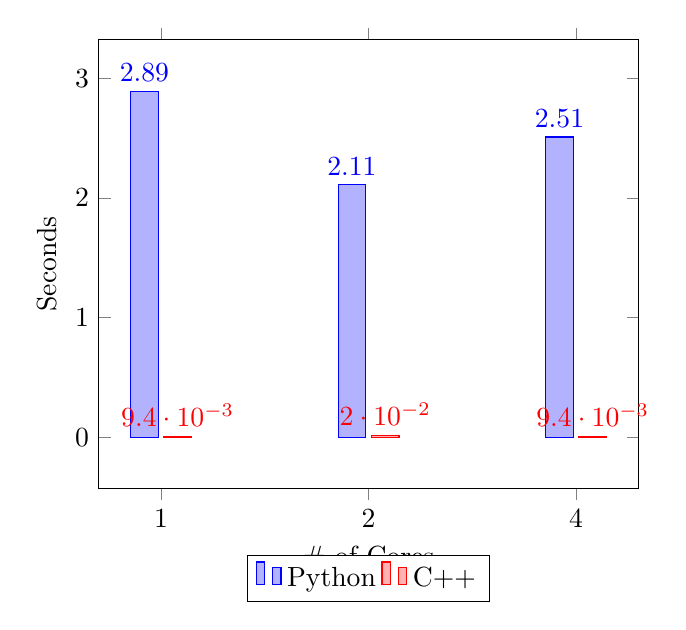
\begin{tikzpicture}
\begin{axis}[
 ybar,
    enlargelimits=0.15,
    legend style={at={(0.5,-0.15)},
      anchor=north,legend columns=-1},
    ylabel={Seconds},
    symbolic x coords={1,2,4},
    xtick=data,
    nodes near coords,
    nodes near coords align={vertical},
    xlabel={\# of Cores}
]	
\addplot coordinates {(1, 2.89) (2, 2.11) (4, 2.51)};
\addplot coordinates {(1, .0094) (2, .02) (4, .0094)};
\legend{Python, C++}
\end{axis}
\end{tikzpicture}

Looking at these results they are very odd. With python having more cores does decrease the amount of time from a single core. However once it is split into 4 cores it takes more time. We assume this is because the code breaks the operations into more threads at each merge step so two threads were being used to do one recursive step and two more threads are doing all rest of them. This combined with the time it takes to start a new thread are most likely the reason the time went up using more cores. \newline

For the C++ code the time increased then went back down most likely because of the thread start cost versus the amount of work they can put in which took it down once there were more cores being applied. 

\end{document}
